\documentclass[12pt,a4paper]{report}
\usepackage[utf8]{vietnam}
\usepackage[top=20mm,right=20mm,bottom=20mm,left=30mm]{geometry}
\usepackage[unicode]{hyperref}
\usepackage{color,fancybox,fancyhdr,graphicx,indentfirst,listings,tikz}

\pagestyle{fancy}
\fancyhf{}
\fancyhead[R]{\textit{LUẬN VĂN TỐT NGHIỆP}}
\fancyhead[L]{\textit{NGUYỄN PHƯỚC THỊNH}}
\fancyfoot[R]{\textit{TRANG \thepage}}
\fancyfoot[L]{\textit{\leftmark}}

\renewcommand{\headrulewidth}{1pt}
\renewcommand{\footrulewidth}{1pt}
\renewcommand{\thesection}{\arabic{section}}
\renewcommand{\thechapter}{\Roman{chapter}}

\definecolor{dkgreen}{rgb}{0,0.6,0}
\definecolor{gray}{rgb}{0.5,0.5,0.5}
\definecolor{mauve}{rgb}{0.58,0,0.82} 
\lstset{
	frame=tb,
	aboveskip=3mm,
	belowskip=3mm,
	showstringspaces=false,
	columns=flexible,
	basicstyle={\small\ttfamily},
	numbers=none,
	numberstyle=\tiny\color{gray},
	keywordstyle=\color{blue},
	commentstyle=\color{dkgreen},
	stringstyle=\color{mauve},
	breaklines=true,
	breakatwhitespace=true,
	tabsize=2
}

\begin{document}
% Trang bìa
\begin{titlepage}
	\setlength{\headheight}{0pt}
	\begin{tikzpicture}[overlay]
		\draw[line width=2pt] (-30pt,10pt) rectangle (\textwidth,-\textheight);
	\end{tikzpicture}
	\begin{center}
		\large ĐẠI HỌC QUỐC GIA TP.HCM\\TRƯỜNG ĐẠI HỌC BÁCH KHOA\\KHOA KHOA HỌC \& KỸ THUẬT MÁY TÍNH
	\end{center}
	\begin{figure}[!ht]
		\begin{center}
			
\includegraphics[width=60mm]{images/logobk.jpg}
		\end{center}
	\end{figure}
	\begin{center}
		\textbf{\large LUẬN VĂN TỐT NGHIỆP ĐẠI HỌC}
	\end{center}
	\vspace{5mm}
	\begin{center}
		\textbf{\Huge ỨNG DỤNG PYTHON VÀO\\LẬP TRÌNH WEBSITE\\ĐÁNH GIÁ SEO}
	\end{center}
	\vspace{5mm}
	\begin{table}[!ht]
		\raggedleft
		\large
		\begin{tabular}{rl}
			\textbf{GVHD:} & TS. NGUYỄN ĐỨC THÁI\\
			\textbf{GVPB:} & ThS. NGUYỄN HỒNG NAM\\
			\\
			\textbf{SVTH:} & NGUYỄN PHƯỚC THỊNH (1413785)\\
		\end{tabular}
	\end{table}
	\vfill
	\begin{center}
		\large TP. HỒ CHÍ MINH, THÁNG \the\month /\the\year
	\end{center}
\end{titlepage}
% Trang cảm ơn
% Lời cam đoan
\begin{center}
    \Large{\textbf{LỜI CAM ĐOAN}}
\end{center}
\vspace{10mm}
\par
Tôi xin cam đoan đây là công trình nghiên cứu đề tài của riêng tôi. Các tài liệu, kết luận được sử dụng trong luận văn có nguồn gốc rõ ràng, đã công bố theo đúng quy định. Đây là đề tài do chính tôi thực hiện và chưa từng sử dụng để nộp lấy bằng cấp ở những nơi khác.
\vspace{1em}
\par
Tôi xin hoàn toàn chịu trách nhiệm về lời cam đoan này.
\vspace{10mm}
\begin{table}[!ht]
    \raggedleft
    \begin{tabular}{c}
        TP. Hồ Chí Minh, Tháng 06/2019\\
        Sinh viên thực hiện\\
        \vspace{5mm}\\
        Nguyễn Phước Thịnh\\
    \end{tabular}
\end{table}
% Lời cảm ơn
\thispagestyle{empty}
\cleardoublepage
\begin{center}
    \Large{\textbf{LỜI CẢM ƠN}}
\end{center}
\vspace{10mm}
\par
Trân trọng gửi lời cảm ơn đến Khoa Khoa học \& Kỹ thuật Máy tính, trường Đại học Bách Khoa TP. Hồ Chí Minh đã tạo điều kiện thuận lợi để tôi có thể học tập tốt và hoàn thành đề tài luận văn này.
\vspace{1em}
\par
Đặc biệt, xin bày tỏ lòng biết biết ơn sâu sắc đến thầy Nguyễn Đức Thái đã hướng dẫn chỉ dạy tôi trong quá trình thực hiện đề tài. Bên cạnh đó, thầy Nguyễn Hồng Nam đã tận tình giúp tôi khắc phục những thiếu sót để tôi có thể hoàn thiện bài luận văn của mình.
\vspace{1em}
\par
Tôi cũng không quên cảm ơn đến gia đình, bạn bè xung quanh đã ủng hộ và giúp tôi có động lực trong suốt thời gian thực hiện đề tài.
\vspace{1em}
\par
Trong quá trình thực hiện luận văn, mặc dù đã cố gắng hoàn thiện đề tài, trao đổi và tiếp thu ý kiến từ các thầy hướng dẫn, tuy nhiên chắc chắn không tránh khỏi những sai sót. Vì vậy tôi mong nhận được sự thông cảm và góp ý chân thành từ mọi người để tôi có thể hoàn thiện trong những đề tài tiếp theo.
\vspace{1em}
\par
Xin chân thành cảm ơn!
\vspace{10mm}
\begin{table}[!ht]
    \raggedleft
    \begin{tabular}{c}
        TP. Hồ Chí Minh, Tháng 06/2019\\
        Sinh viên thực hiện\\
        \vspace{5mm}\\
        Nguyễn Phước Thịnh\\
    \end{tabular}
\end{table}
\thispagestyle{empty}
\cleardoublepage
% Tóm tắt
\begin{center}
    \Large{\textbf{TÓM TẮT}}
\end{center}
\vspace{10mm}
\par
Với sự phát triển không ngừng của Internet và độ phổ biến của nó trên toàn thế giới, việc khai thác nội dung số để quảng bá website của mình đến với người dùng là hết sức quan trọng. Tuy nhiên, làm thế nào để có thể tiếp cận với số đông người dùng là việc làm không hề đơn giản. Mục tiêu là tăng khả năng xuất hiện khi người dùng tìm kiếm nội dung liên quan đến website của mình, gồm tập hợp các phương pháp nhằm cải thiện thứ hạng website trên trang kết quả tìm kiếm, hay còn gọi là tối ưu hóa công cụ tìm kiếm (Search Engine Optimization - SEO).
\vspace{1em}
\par
Do đó, chúng tôi quyết định nghiên cứu về đề tài này và xây dựng nên công cụ tự động phân tích mã nguồn website theo các tiêu chuẩn SEO hiện có, sau đó hiển thị kết quả đánh giá giúp người dùng có thể tối ưu website của họ.
\vspace{1em}
\par
Những nội dung chính sẽ được trình bày trong luận văn:
\begin{itemize}
    \item Chương I: Giới thiệu đề tài
    \item Chương II: Nền tảng lý thuyết
    \item Chương III: Các tiêu chuẩn SEO
    \item Chương IV: Thiết kế giải pháp
    \item Chương V: Hiện thực
    \item Chương VI: Kết luận đánh giá
\end{itemize}
\thispagestyle{empty}
\cleardoublepage

\setlength{\headheight}{18pt}

\newpage
\tableofcontents
\listoftables
\listoffigures
\newpage

\setlength{\parskip}{1em}

% Giới thiệu đề tài
\chapter{Giới thiệu đề tài}
\section{Tính cấp thiết}
Với sự lớn mạnh không ngừng của Internet và độ phổ biến của nó trên toàn Thế giới, việc các doanh nghiệp và cửa hành kinh doanh sử dụng nó để mang lại doanh thu cho mình là hết sức quan trọng. Tuy nhiên, có rất nhiều đơn vị muốn chiếm lĩnh vị trí cao trên nó dẫn đến việc cạnh tranh rất gay gắt trong công cuộc đưa website của mình đến với đại đa số khách hàng ở khắp mọi nơi, được gọi tắt là SEO (Search Engine Optimization).
\\\par
Từ đó việc tối ưu trang web để mang lại thứ hạng cao trên các công cụ tìm kiếm ra đời. Người lập trình viên ngoài việc phải đáp ứng các kịch bản của ứng dụng mà còn phải đảm bảo tối ưu website của họ đối với các công cụ tìm kiếm. Để giúp cho công việc của họ được thuận tiện hơn và tuân thủ được các tiêu chí tối ưu mới nhất, chúng tôi cung cấp một giải pháp tự động, phân tích cú pháp trang web và đưa ra những đề nghị sửa chữa, nhằm tối ưu SEO cho trang web của họ.
\section{Mục tiêu}
Để mang đến sự thuận tiện và hài lòng cho người sử dụng, ứng dụng của chúng tôi sẽ đặt ra những mục tiêu sau đây:
\begin{itemize}
	\item Cung cấp dịch vụ đánh giá miễn phí và sẽ luôn miễn phí! Vì thế chúng tôi sẽ đặt quảng cáo lên trang web để mang lại nguồn thu duy trì cho chúng tôi.
	\item Cập nhật những tiêu chuẩn về SEO đến người dùng thông qua các bài viết trên website và đảm bảo rằng công cụ của chúng tôi sẽ sử dụng những tiêu chuẩn mới nhất.
	\item Tự động phân tích cú pháp trang web người dùng, so sánh với các tiêu chuẩn về SEO, đưa ra kết quả, đánh giá và gợi ý cho người dùng cách để họ có thể khắc phục nếu website chưa đạt chuẩn hoặc thiếu các thành phần quan trọng.
	\item Để tránh việc lặp lại kiểm tra cho cùng một trang web, chúng tôi sẽ lưu lại kết quả đánh giá và hiển thị ra nếu người dùng kiểm tra cùng một địa chỉ. Sau 24h, chúng tôi sẽ cập nhật kết quả mới khi người dùng cần kiểm tra lại.
\end{itemize}
\section{Phương pháp thực hiện}
Chúng tôi sử dụng Python để làm ngôn ngữ lập trình cốt lõi cho ứng dụng của mình. Python được biết đến là ngôn ngữ dành cho tính toán và phân tích nên sẽ thích hợp để xử lý các cú pháp cho trang web chúng tôi cần kiểm tra.
\\\par
Cụ thể hơn, sau đây là những framework và thư viện chúng tôi sẽ sử dụng cho ứng dụng của mình:
\begin{itemize}
	\item Django: Framework Python dùng để phát triển ứng dụng web.
	\item Requests, Lxml: Thư viện Python có nhiệm vụ phân tích cú pháp và lấy từng phần tử của website chúng tôi cần kiểm tra.
	\item reCAPTCHA: Ứng dụng do Google phát triển, nhằm hạn chế spam và BOT tác động lên website để giữ trang web trở nên an toàn.
	\item Bootstrap: Thư viện dùng để thiết kế giao diện cho trang web của chúng tôi, nó hỗ trợ tốt cho việc hiển thị website đa nền tảng.
	\item Font Awesome: Thư viện cung cấp các icon cần thiết cho giao diện website.
	\item Heroku: Cloud platform miễn phí để chúng tôi triển khai ứng dụng Python của mình lên Internet.
\end{itemize}
\section{Bố cục báo cáo}
Tiếp theo, những phần sau chúng tôi sẽ trình bày cách chúng tôi sử dụng những framework và thư viện để xây dựng nên website cùng với những tiêu chí được áp dụng để đánh giá SEO cho một trang web. Phần kết luận đánh giá sẽ được thông tin vào mục cuối cùng kèm theo những tài liệu tham khảo mà chúng tôi sử dụng để hoàn thành báo cáo này.
% Nền tảng lý thuyết
\chapter{Nền tảng lý thuyết}
Phần này chúng tôi sẽ giới thiệu cũng như trang bị những kiến thức cơ bản để sử dụng những công cụ được liệt kê ở phần trước.
\section{Ngôn ngữ Python}
Python hiện đang là một trong những ngôn ngữ lập trình phổ biến. Một phần nhờ vào khả năng dễ tiếp cận, cấu trúc rõ ràng và quan trọng hơn, nó có thể giải quyết tốt các bài toán kỹ thuật với thời gian thực thi nhanh và tiết kiệm dòng code. Python được tạo ra bởi Guido van Rossum và phát hành vào năm 1991.\cite{python}
\par
Phiên bản sử dụng: 3.7.3
\begin{itemize}
	\item Biến (Variable): Không giống với các ngôn ngữ khác, Python không có câu lệnh riêng biệt để khai báo biến. Biến không cần phải khai báo kiểu giá trị nào và có thể thay đổi dựa vào giá trị mà nó được gán.
	\begin{lstlisting}[language=Python]
# x is of type int
x = 5
# x is now of type str
x = "Thinh"
	\end{lstlisting}
	\item Chuỗi (String): Chuỗi ký tự trong Python được chứa trong cặp dấu nháy đơn hoặc dấu nháy kép. Để hiển thị chuỗi ra màn hình, sử dụng lệnh \texttt{print()}.
	\begin{lstlisting}[language=Python]
a = "Hello, World!"
print(a)

>>>"Hello, World"
	\end{lstlisting}
	\item Toán tử (Operator):
	\begin{itemize}
		\item Số học:
		\begin{table}[!ht]
			\centering
			\begin{tabular}{|c|l|}
				\hline
				$+$ & Cộng\\
				\hline
				$-$ & Trừ\\
				\hline
				$*$ & Nhân\\
				\hline
				$/$ & Chia\\
				\hline
				$\%$ & Chia lấy phần dư\\
				\hline
				$**$ & Lũy thừa\\
				\hline
				$//$ & Chia lấy phần nguyên\\
				\hline
			\end{tabular}
			\caption{Toán tử Số học}
		\end{table}
		\item So sánh:
		\begin{table}[!ht]
			\centering
			\begin{tabular}{|c|l|}
				\hline
				$==$ & Bằng\\
				\hline
				$!=$ & Không bằng\\
				\hline
				$>$ & Lớn hơn\\
				\hline
				$<$ & Nhỏ hơn\\
				\hline
				$>=$ & Lớn hơn hoặc bằng\\
				\hline
				$<=$ & Nhỏ hơn hoặc bằng\\
				\hline
			\end{tabular}
			\caption{Toán tử So sánh}
		\end{table}
		\item Logic:
		\begin{table}[!ht]
			\centering
			\begin{tabular}{|c|l|}
				\hline
				$and$ & Trả về \texttt{True} nếu 2 điều kiện đều đúng\\
				\hline
				$or$ & Trả về \texttt{True} nếu 1 trong 2 điều kiện là đúng\\
				\hline
				$not$ & Đảo ngược kết quả của điều kiện\\
				\hline
			\end{tabular}
			\caption{Toán tử Logic}
		\end{table}
		\item Identity:
		\begin{table}[!ht]
			\centering
			\begin{tabular}{|c|l|}
				\hline
				$is$ & Trả về \texttt{True} nếu 2 biến cùng trỏ tới 1 đối tượng\\
				\hline
				$is$ $not$ & Trả về \texttt{True} nếu 2 biến không trỏ cùng đối tượng\\
				\hline
			\end{tabular}
			\caption{Toán tử Identity}
		\end{table}
		\item Membership:
		\begin{table}[!ht]
			\centering
			\begin{tabular}{|c|l|}
				\hline
				$in$ & Trả về \texttt{True} nếu biến nằm trong tập hợp các biến\\
				\hline
				$not$ $in$ & Trả về \texttt{True} nếu biến không nằm trong tập hợp các biến\\
				\hline
			\end{tabular}
			\caption{Toán tử Membership}
		\end{table}
	\end{itemize}
	\item Dictionary: Tập hợp không có thứ tự, có thể thay đổi và lập chỉ mục. Được biểu diễn bằng cặp dấu ngoặc nhọn, bên trong là khóa (key) và giá trị (value) tương ứng.
	\begin{lstlisting}[language=Python]
hoten = {
	"ho": "Nguyen Phuoc",
	"ten": "Thinh"
}
	\end{lstlisting}
	\item Câu điều kiện (If\ldots Else): Dùng để thực thi một hành động sau khi thỏa điều kiện cho trước. Lưu ý trong Python, sử dụng thụt lề dòng để phân biệt các khối lệnh với nhau.
	\begin{lstlisting}[language=Python]
a = 1
b = 2
if a > b:
	print("a is greater than b")
elif a == b:
	print("a and b are equal")
else:
	print("b is greater than a")

>>>"b is greater than a"
	\end{lstlisting}
	\item Vòng lặp (For): Dùng để lặp qua một chuỗi (có thể là list, tuple, dictionary, set hoặc string).
	\begin{lstlisting}[language=Python]
hoten = ["Nguyen", "Phuoc", "Thinh"]
for x  in hoten:
	print(x)
	
>>>"Nguyen"
>>>"Phuoc"
>>>"Thinh"
	\end{lstlisting}
	\item Hàm (Function): Gồm một khối code, được khởi chạy khi được gọi đến. Để truyền dữ liệu vào 1 hàm được gọi là tham số (parameter). Hàm trả về kết quả thông qua lệnh \texttt{return}.
	\begin{lstlisting}[language=Python]
# a function is defined using the def keyword
def add(n):
	return 1 + n
# calling a function
add(1)

>>>2
	\end{lstlisting}
	\item Lớp/Đối tượng (Class/Object): Python là ngôn ngữ lập trình hướng đối tượng. Hầu hết mọi thứ trong Python là một đối tượng (object), gồm thuộc tính và phương thức của nó. Sử dụng lớp (class) để khởi tạo 1 đối tượng mới.
	\begin{lstlisting}[language=Python]
# create a class
class Person:
	def __init__(self, name, age):
		self.name = name
		self.age = age
	# object method
	def func(self):
		print(f"My name is: {self.name}, {self.age} years old")
# create object
p = Person("Thinh", 20)
p.func()
# modify object property
p.age = 22
print(p.age)

>>>"My name is: Thinh, 20 years old"
>>>22
	\end{lstlisting}
	\item Module: Có thể xem module là 1 bộ thư viện mã code, được lưu bởi tệp hoặc thư mục tách biệt với project đang thực thi, được nhúng vào để tái sử dụng những bộ code chứa trong đó.
	\par
	Để sử dụng các hàm hoặc lớp trong file \texttt{mymodule.py}, ta sử dụng lệnh sau:
	\begin{lstlisting}[language=Python]
import mymodule
# import only part from a module
from mymodule import myfunc
	\end{lstlisting}
	\item PIP: Là trình quản lý gói (package) hoặc module dành cho Python. Gói là nơi chứa tất cả các file cần thiết cho 1 module.
	\par
	Để cài đặt 1 gói trong Python, sử dụng lệnh sau:
	\begin{lstlisting}[language=bash]
\>pip install Django
	\end{lstlisting}
	\item Xử lý ngoại lệ (Try\ldots Except): Khi chương trình xảy ra lỗi hoặc ngoại lệ, Python sẽ dừng lại và đưa ra thông báo lỗi cho người dùng. Để tránh ứng dụng bị gián đoạn, sử dụng câu lệnh \texttt{try} để bắt và xử lý các ngoại lệ khi chương trình đang được thực thi.
	\begin{lstlisting}[language=Python]
try:
	print(x)
except NameError:
	print("Variable x is not defined")
	
>>>"Variable x is not defined"
	\end{lstlisting}
\end{itemize}
\section{Framework Django}
Django là 1 framework Python web cấp cao, thúc đẩy phát triển nhanh chóng, gọn gàng và tiện dụng. Được xây dựng bởi các nhà lập trình viên có kinh nghiệm, xử lý được các vấn đề rắc rối khi phát triển web, do đó người dùng chỉ cần quan tâm hoàn thiện các chức năng cho web mà không cần phải quá lo lắng về nền tảng phía sau. Và quan trọng nó là mã nguồn mở và miễn phí.
\par
Chúng tôi sẽ sử dụng mục tài liệu\cite{django} tại trang chủ của Django framework để trình bày những khái niệm và cách để hiện thực ứng dụng của chúng tôi.
\par
Phiên bản sử dụng: 2.1.4
\begin{itemize}
	\item Sau khi cài đặt xong Django từ trình quản lý gói PIP của Python, dùng lệnh sau để khởi tạo project mới có tên là \texttt{lvtn}:
	\begin{lstlisting}[language=bash]
\>django-admin startproject lvtn
	\end{lstlisting}
	Một folder mới được tạo ra chứa các thành phần của project, có cấu trúc và chức năng như sau:
	\begin{lstlisting}[language=bash]
lvtn\
	lvtn\
		__init__.py
		settings.py
		urls.py
		wsgi.py
	manage.py
	\end{lstlisting}
	\begin{itemize}
		\item \texttt{manage.py}: Một CLI giúp tương tác với ứng dụng web.
		\item \texttt{lvtn\textbackslash\_\_init\_\_.py}: File rỗng, để chỉ cho Python biết thư mục này nên được xem là một gói.
		\item \texttt{lvtn\textbackslash settings.py}: Chứa các tùy chỉnh của project.
		\item \texttt{lvtn\textbackslash urls.py}: Các khai báo URL cho trang web.
		\item \texttt{lvtn\textbackslash wsgi.py}: Được sử dụng khi deploy project lên Internet.
	\end{itemize}
	\item Server phát triển: Dùng để khởi chạy ứng dụng web trên máy tính local.
	\begin{lstlisting}[language=bash]
\>python manage.py runserver
	\end{lstlisting}
	Khi server đang chạy, truy cập vào địa chỉ \url{http://127.0.0.1:8000} trên trình duyệt web để thấy ứng dụng đang được trình diễn.
	\item Tạo app mới: Mỗi ứng dụng được viết trong Django bao gồm 1 gói Python tuân thủ theo 1 quy ước nhất định. Django đi kèm với 1 tiện ích tự động tạo cấu trúc thư mục cơ bản của 1 ứng dụng, do đó người lập trình chỉ cần quan tâm đến việc phát triển code bên trong mà thôi.
	\par
	Tạo app \texttt{checkweb}	có nhiệm vụ xử lý chính cho project của chúng tôi.
	\begin{lstlisting}[language=bash]
\>python manage.py startapp checkweb
	\end{lstlisting}
	Thư mục mới được tạo ra có cấu trúc như sau:
	\begin{lstlisting}[language=bash]
checkweb\
	migrations\
		__init__.py
	__init__.py
	admin.py
	apps.py
	models.py
	tests.py
	views.py
	\end{lstlisting}
	\begin{itemize}
		\item \texttt{migrations\textbackslash}: Thư mục chứa các file được sinh ra khi có thay đổi về cấu trúc cơ sở dữ liệu.
		\item \texttt{admin.py}: Dùng để thiết đặt các thuộc tính được hiển trị trong trang quản trị admin mà Django cung cấp sẵn.
		\item \texttt{apps.py}: Khai báo app được sử dụng trong project, đảm bảo rằng các app không bị trùng lặp trong 1 dự án.
		\item \texttt{models.py}: Django hỗ trợ các phương thức để xử lý cơ sở dữ liệu mà không cần sử dụng đến các câu lệnh truy vấn SQL trực tiếp.
		\item \texttt{tests.py}: Được người dùng sử dụng để triển khai các kịch bản thử nghiệm và rà soát lỗi trước khi phát hành ứng dụng.
		\item \texttt{views.py}: Đóng vai trò xử lý trung tâm của ứng dụng, quản lý việc hiển thị, kết nối đến cơ sở dữ liệu và thực thi các hàm do lập trình viên thêm vào ứng dụng.
		\par
		Sau khi tạo xong app, cần phải khai báo trong project bằng các thêm dòng sau vào file \texttt{lvtn\textbackslash settings.py}:
		\begin{lstlisting}[language=Python]
INSTALLED_APPS = [
    "django.contrib.admin",
    "django.contrib.auth",
    "django.contrib.contenttypes",
    "django.contrib.sessions",
    "django.contrib.messages",
    "django.contrib.staticfiles",
    # add code below
    "checkweb.apps.CheckwebConfig",
]
	\end{lstlisting}
	\end{itemize}
	\item Migration: Khi tạo mới hoặc có sự thay đổi về cấu trúc cơ sở dữ liệu, migration có nhiệm vụ lưu lại quá trình ứng dụng thay đổi, do đó có thể truy vết lại và phục hồi lại những cập nhật trước đó 1 cách dễ dàng, nhất là khi ứng dụng gặp lỗi. Để thực hiện, dùng các lệnh sau:
	\begin{lstlisting}[language=bash]
\>python manage.py migrate
\>python manage.py makemigrations
\>python manage.py migrate
	\end{lstlisting}
	\item Trang quản trị admin: Một trong những ưu điểm của Django so với các framework khác là nó cung cấp trang Django administration giúp hiển trị trực quan cơ sở dữ liệu do người dùng thiết lập, cho phép xem, tạo mới, chỉnh sửa, xóa và nhiều tính năng khác nữa.
	\par
	Để có thể truy cập vào trang quản trị thì trước tiên cần phải tạo tài khoản \texttt{superuser}:
	\begin{lstlisting}[language=bash]
\>python manage.py createsuperuser
\>Username: ___
\>Email address: ___
\>Password: ___
\>Password (again): ___
\>Superuser created successfully.
	\end{lstlisting}
	Sau khi điền đầy đủ các thông tin trên thì có thể đăng nhập tài khoản để truy cập vào trang quản trị tại địa chỉ: \url{http://127.0.0.1:8000/admin/}
	\item Class-based view: Đây là chức năng được Django hỗ trợ, giúp lập trình viên ít phải viết code hơn để hiện thị 1 giao diện lên trình duyệt web. Nó hỗ trợ tốt trong việc truyền tham số, lấy giá trị từ model và có thể dễ dàng tùy chỉnh theo ý muốn.
	\par
	Để sử dụng, cần phải thêm module vào file muốn dùng nó. Đoạn code sau có chức năng hiển thị file \texttt{about.html} ra đường dẫn \url{http://127.0.0.1:8000/about/}.
	\begin{lstlisting}[language=Python]
from django.urls import path
from django.views.generic import TemplateView

urlpatterns = [
	path("about/", TemplateView.as_view(template_name="about.html")),
]
	\end{lstlisting}
	\item Django template: Dựa trên file \texttt{.html} nhưng có chèn thêm các đoạn code riêng biệt để mỗi khi chạy chương trình, Django sẽ render ra giao diện lên trình duyệt tương ứng.
	\begin{lstlisting}[language=HTML]

{{ section.title }}

<h1>{{ section.title }}</h1>

<h2>
 	<a href="{{ story.get_absolute_url }}">
		{{ story.headline|upper }}
	</a>
</h2>
<p>{{ story.tease|truncatewords:100 }}</p>


	\end{lstlisting}
\end{itemize}
\section{Thư viện Python}
\subsection{Requests}
Tham khảo\cite{requests}.
\par
Phiên bản sử dụng: 2.21.0
\begin{itemize}
	\item Cách cài đặt:
	\begin{lstlisting}[language=bash]
\>pip install requests
	\end{lstlisting}
	\item Phương thức \texttt{get}: Dùng để 	lấy toàn bộ nội dung trang web dựa trên tham số url.
	\begin{lstlisting}[language=Python]
import requests
page = requests.get(url)
	\end{lstlisting}
\end{itemize}
\subsection{Lxml}
Tham khảo\cite{lxml}.
\par
Phiên bản sử dụng: 4.3.3
\begin{itemize}
	\item Cách cài đặt:
	\begin{lstlisting}[language=bash]
\>pip install lxml
	\end{lstlisting}
	\item Gói \texttt{lxml.html}: Dùng để phân tách chuỗi HTML.
	\begin{lstlisting}[language=Python]
from lxml import html
content = html.fromstring(page.content)
value = content.xpath("//title/text()")
	\end{lstlisting}
\end{itemize}
\section{Thư viện giao diện}
\subsection{Bootstrap}
Tham khảo\cite{bootstrap}.
\par
Phiên bản sử dụng: 4.3.1
\begin{itemize}
 	\item CSS: Sao chép và dán dòng code bên dưới vào trong thẻ \texttt{<head>} trước tất cả các định dạng khác để tải CSS của Bootstrap.
 	\begin{lstlisting}[language=HTML]
<link rel="stylesheet" href="https://stackpath.bootstrapcdn.com/bootstrap/
4.1.3/css/bootstrap.min.css">
	\end{lstlisting}
	\item JS: Đặt trong thẻ \texttt{<script>} ở gần cuối trang web, trước khi đóng thẻ \texttt{</body>} để kích hoạt chúng. jQuery phải được đặt trước, đến Popper.js và sau cùng là phần JavaScript.
	\begin{lstlisting}[language=HTML]
<script src="https://code.jquery.com/jquery-3.3.1.slim.min.js"></script>
<script src="https://cdnjs.cloudflare.com/ajax/libs/popper.js/1.14.3/umd/
popper.min.js"></script>
<script src="https://stackpath.bootstrapcdn.com/bootstrap/4.1.3/js/
bootstrap.min.js"></script>
	\end{lstlisting}
\end{itemize}
\subsection{Font Awesome}
Tham khảo\cite{awesome}.
\par
Phiên bản sử dụng: 5.8.2
\par
Trước khi sử dụng được, cần phải chèn dòng code bên dưới vào thẻ \texttt{<head>} nằm ở đầu trang web.
\begin{lstlisting}[language=HTML]
<link rel="stylesheet" href="https://use.fontawesome.com/releases/v5.5.0/css/
all.css">
\end{lstlisting}
\par
Để chèn icon vào trang web, sử dụng dòng code tương tự cú pháp bên dưới:
\begin{lstlisting}[language=HTML]
<i class="fas fa-heart"></i>
\end{lstlisting}
\section{Bảo mật}
\subsection{reCAPTCHA}
Tham khảo\cite{captcha}.
\par
Phiên bản sử dụng: reCAPTCHA v2
\par
Cách đơn giản để sử dụng reCAPTCHA vào trang web bằng cách nhúng mã JavaScript và thẻ \texttt{g-recaptcha}. Thẻ \texttt{g-recaptcha} là 1 thẻ \texttt{DIV} với tên class là \texttt{"g-recaptcha"}, có thuộc tính \texttt{data-sitekey} chứa Site key được cấp khi đăng ký sử dụng reCAPTCHA.
\begin{lstlisting}[language=HTML]
<html>
	<head>
		<title>reCAPTCHA demo: Simple page</title>
		<script src="https://www.google.com/recaptcha/api.js" async defer></script>
	</head>
	<body>
		<form action="?" method="POST">
			<div class="g-recaptcha" data-sitekey="your_site_key"></div>
			<br/>
			<input type="submit" value="Submit">
		</form>
	</body>
</html>
\end{lstlisting}
\par
Sau khi submit form sử dụng reCAPTCHA, cần phải gửi giá trị có tên là \texttt{g-recaptcha-\\response} bằng phương thức POST về máy chủ của Google để xác minh người dùng đã xác thực bằng reCAPTCHA tại địa chỉ \url{https://www.google.com/recaptcha/api/siteverify}.
\begin{itemize}
	\item secret (bắt buộc): Khóa Secret key được cấp đồng thời với Site key khi đăng ký sử dụng.
	\item response (bắt buộc): Kết quả trả về của thuộc tính có tên là \texttt{g-recaptcha-response}.
	\item remoteip: Địa chỉ IP của người dùng cuối.
\end{itemize}
\par
Tiếp theo, Google sẽ trả về kết quả kiểm tra có thỏa reCAPTCHA dưới dạng JSON bằng các giá trị sau:
\begin{lstlisting}[language=Python]
{
	"success": true|false,
	"challenge_ts": timestamp, # timestamp of the challenge load
	"hostname": string, # the hostname of the site where the reCAPTCHA was solved
	"error-codes": [...] # optional
}
\end{lstlisting}
\par
Dựa vào kết quả này, chúng tôi có thể biết được người dùng đã có giải được captcha hay chưa, sau đó tiến hành các yêu cầu từ người dùng.	
\section{Triển khai ứng dụng}
\subsection{Heroku platform}
Tham khảo\cite{heroku}.
\par
Đầu tiên và quan trọng nhất, các ứng dụng Heroku yêu cầu 1 file \texttt{Procfile} để cài đặt nền tảng sử dụng, được đặt tại thư mục gốc.
\par
\texttt{Procfile}
\begin{lstlisting}[language=sh]
web: gunicorn myproject.wsgi
\end{lstlisting}
\par
File \texttt{Procfile} này yêu cầu \texttt{Gunicorn}, 1 máy chủ web được khuyến nghị dùng cho ứng dụng Django. Để cài đặt, sử dụng lệnh:
\begin{lstlisting}[language=bash]
\>pip install gunicorn
\end{lstlisting}
\par
Thay đổi trong file \texttt{settings.py} của ứng dụng Django. Khi sử dụng Heroku, các thông tin nhạy cảm sẽ được lưu trữ trong môi trường được gọi là config vars. Nó bao gồm các thông tin để kết nối đến cơ sở dữ liệu, trong khi bình thường sẽ được ghi trong file \texttt{settings.py} của Django.
\par
Gói \texttt{django-heroku} sẽ tự động cấu hình ứng dụng Django để nó hoạt động trên Heroku. Nó tương thích với các ứng dụng Django 2.0. Để cài đặt, sử dụng lệnh:
\begin{lstlisting}[language=bash]
\>pip install django-heroku
\end{lstlisting}
\par
Sau khi cài đặt, cần phải \texttt{import} câu lệnh sau vào đầu file \texttt{settings.py}:
\begin{lstlisting}[language=Python]
import django_heroku
\end{lstlisting}
\par
Sau đó thêm phần sau vào cuối file \texttt{settings.py}:
\begin{lstlisting}[language=Python]
# activate django-heroku.
django_heroku.settings(locals())
\end{lstlisting}
\par
Triển khai ứng dụng và hoàn tất.
% Các tiêu chuẩn seo
\chapter{Các tiêu chuẩn SEO}
Để thu hút khách hàng truy cập và sử dụng một webstie, có rất nhiều tiêu chí như giao diện đẹp, tốc độ đáp ứng nhanh, thiết kế thuận tiện nhằm mang đến trải nghiệm tốt cho người dùng. Các vấn đề trên là một trong những tiêu chí mà công cụ tìm kiếm dùng để đánh giá website xem có phù hợp mà từ đó đề xuất lên trang kết quả khi có người dùng tìm kiếm dựa trên nội dung có liên quan.
\par
Bên cạnh đó, việc xây dựng một website có cấu trúc phù hợp, sẽ giúp thể hiện rõ ràng nội dung khi các công cụ tìm kiếm phân tích website, qua đó nâng thứ hạng website trên trang kết quả tìm kiếm. Điều này sẽ khiến người dùng dễ dàng tiếp cận và truy cập vào website của mình. Ứng dụng của chúng tôi được tạo ra nhằm phân tích cú pháp SEO của một website, giúp người dùng tìm ra những thiếu sót về cú pháp trong SEO và sau đó cải thiện chúng.
\par
Sau đây là các tiêu chuẩn cần thiết cho một website chuẩn SEO về mặt cú pháp, chúng tôi tham khảo bài viết từ trang \href{https://moz.com/}{moz.com} là một trong những dịch vụ phân tích SEO uy tín và được thành lập từ năm 2004\cite{seo}:
\section{Thẻ header}
Thẻ tiêu đề là một yếu tố HTML được sử dụng để chỉ định các tiêu đề trên trang của bạn. Thẻ tiêu đề chính, được gọi là \textbf{\texttt{h1}}, thường được dành riêng cho tiêu đề của trang. Nó trông như thế này:
\begin{lstlisting}[language=html]
<h1>Tieu de trang</h1>
\end{lstlisting}
\par
Ngoài ra còn có các tiêu đề phụ đi từ thẻ \textbf{\texttt{h2}} đến \textbf{\texttt{h6}}, mặc dù không cần sử dụng tất cả các tiêu đề này trên một trang. Hệ thống phân cấp của các thẻ tiêu đề đi từ \textbf{\texttt{h1}} đến \textbf{\texttt{h6}} theo thứ tự quan trọng giảm dần.
\par
Mỗi trang nên có một \textbf{\texttt{h1}} duy nhất mô tả chủ đề chính của trang, điều này thường được tạo tự động từ tiêu đề của trang. Là tiêu đề mô tả chính của trang, \textbf{\texttt{h1}} nên chứa từ khóa hoặc cụm từ chính của trang đó.
\par
Chủ đề chính của trang được giới thiệu trong tiêu đề \textbf{\texttt{h1}} và mỗi tiêu đề bổ sung được sử dụng để giới thiệu một chủ đề phụ mới. Ví dụ, \textbf{\texttt{h2}} cụ thể hơn \textbf{\texttt{h1}} và các thẻ \textbf{\texttt{h3}} cụ thể hơn so với \textbf{\texttt{h2}}.
\section{Liên kết nội bộ}
Một phần của trang web có khả năng thu thập dữ liệu nằm trong cấu trúc liên kết nội bộ của nó. Khi bạn liên kết đến các trang khác trên trang web của mình, bạn đảm bảo rằng trình thu thập thông tin của công cụ tìm kiếm có thể tìm thấy tất cả các trang của bạn và giúp khách truy cập điều hướng trang web của bạn.
\section{Văn bản neo}
Văn bản neo là văn bản mà bạn liên kết đến các trang. Dưới đây, bạn có thể thấy một ví dụ về những gì một liên kết không có văn bản neo và một liên kết với văn bản neo sẽ trông như thế nào trong HTML.
\begin{lstlisting}[language=html]
<a href="http://www.example.com"></a>
<a href="http://www.example.com" title="Keyword Text">Keyword Text</a>
\end{lstlisting}
\par
Trên chế độ xem trực tiếp, nó sẽ trông như thế này:
\begin{lstlisting}
http://www.example.com
Keyword Text
\end{lstlisting}
\par
Văn bản neo gửi tín hiệu đến các công cụ tìm kiếm liên quan đến nội dung của trang đích. Ví dụ, nếu muốn liên kết đến một trang trên trang web bằng cách sử dụng văn bản neo "Học hỏi SEO", thì đó là một chỉ báo tốt cho các công cụ tìm kiếm rằng trang được nhắm mục tiêu là nơi mọi người có thể tìm hiểu về SEO.
\section{Khối lượng liên kết}
Trong Nguyên tắc quản trị trang web chung của Google, họ nói việc giới hạn số lượng liên kết trên một trang ở mức hợp lý (nhiều nhất là vài nghìn). Đây là một phần của hướng dẫn kỹ thuật của Google, thay vì phần hướng dẫn chất lượng, vì vậy có quá nhiều các liên kết nội bộ không phải là điều quá nghiêm trọng, nhưng nó ảnh hưởng đến cách Google tìm và đánh giá các trang của bạn.
\par
Vì vậy, bạn chỉ nên liên kết khi bạn muốn nói điều đó. Quá nhiều liên kết không chỉ làm loãng nội dung của mỗi liên kết, mà chúng còn có thể không có ích và quá sức đối với việc Google hiểu trang của bạn.
\par
Tập trung vào chất lượng và giúp người dùng điều hướng trang web của bạn sẽ có khả năng bạn đã giành chiến thắng mà không phải lo lắng về quá nhiều về số lượng liên kết.
\section{Chuyển hướng}
Xóa và đổi tên trang là một cách phổ biến, nhưng trong trường hợp bạn di chuyển một trang, hãy đảm bảo cập nhật các liên kết đến URL cũ đó. Bạn nên đảm bảo chuyển hướng URL đến vị trí mới của nó, nhưng nếu có thể, hãy cập nhật tất cả các liên kết nội bộ đến URL đó tại nguồn để người dùng và trình thu thập thông tin không phải chuyển hướng đến trang đích. Hãy cẩn thận để tránh các vòng chuyển hướng quá nhiều (theo Google, nên giữ số vòng chuyển hướng không quá 3 và ít hơn 5).
\par
Thay vì:
\begin{lstlisting}
example.com/location1 -> example.com/location2 -> example.com/location3
\end{lstlisting}
\par
Nên dùng:
\begin{lstlisting}
example.com/location1 -> example.com/location3
\end{lstlisting}
\section{Tối ưu hình ảnh}
Hình ảnh là thủ phạm lớn nhất của các trang web chậm. Cách tốt nhất để giải quyết vấn đề này là nén hình ảnh của bạn. Một cách khác để giúp tối ưu hóa hình ảnh của bạn (và cải thiện tốc độ trang) là chọn định dạng hình ảnh phù hợp.
\par
Cách chọn định dạng hình ảnh sẽ sử dụng:
\begin{itemize}
	\item Nếu hình ảnh của bạn là ảnh động, hãy sử dụng GIF.
	\item Nếu bạn không cần giữ độ phân giải hình ảnh cao, hãy sử dụng JPEG (và kiểm tra các cài đặt nén khác nhau).
	\item Nếu bạn cần duy trì độ phân giải hình ảnh cao, hãy sử dụng PNG.
	\begin{itemize}
		\item Nếu hình ảnh của bạn có nhiều màu sắc, hãy sử dụng PNG-24.
		\item Nếu hình ảnh của bạn không có nhiều màu sắc, hãy sử dụng PNG-8.
	\end{itemize}
\end{itemize}
\section{Thuộc tính alt}
Văn bản thay thế trong hình ảnh là một nguyên tắc của khả năng truy cập web và được sử dụng để mô tả khi hình ảnh không thể hiển thị. Điều quan trọng là phải có mô tả văn bản thay thế để có thể hiểu những gì hình ảnh trên trang web của bạn mô tả vấn đề gì.
\par
Các bot công cụ tìm kiếm cũng thu thập dữ liệu văn bản thay thế để hiểu rõ hơn về hình ảnh của bạn, điều này mang lại cho bạn lợi ích bổ sung trong việc cung cấp bối cảnh hình ảnh tốt hơn cho các công cụ tìm kiếm. Chỉ cần đảm bảo rằng các mô tả alt của bạn đọc tự nhiên cho mọi người và tránh nhồi nhét từ khóa cho các công cụ tìm kiếm.
\par
Thay vì:
\begin{lstlisting}[language=html]
<img src="grumpycat.gif" alt="grumpy cat, cat is grumpy, grumpy cat gif">
\end{lstlisting}
\par
Nên dùng:
\begin{lstlisting}[language=html]
<img src="grumpycat.gif" alt="A black cat looking very grumpy at a big spotted dog">
\end{lstlisting}
\section{Định dạng nội dung}
Trang của bạn có thể chứa nội dung tốt nhất từng được viết về một chủ đề, nhưng nếu nó được định dạng không đúng, khán giả của bạn có thể không bao giờ đọc nó. Một số nguyên tắc có thể thúc đẩy khả năng đọc, bao gồm:
\begin{itemize}
	\item Kích thước và màu sắc: tránh các phông chữ quá nhỏ. Google khuyến nghị sử dụng phông chữ 16px trở lên để tối ưu hóa trên điện thoại di động. Màu văn bản liên quan đến màu nền của trang cũng sẽ thúc đẩy khả năng đọc.
	\item Tiêu đề: chia nhỏ nội dung của bạn bằng các tiêu đề hữu ích có thể giúp người đọc điều hướng trang. Điều này đặc biệt hữu ích trên các trang dài, nơi người đọc có thể chỉ tìm kiếm thông tin từ một phần cụ thể.
	\item Ý chính: tuyệt vời cho danh sách, nội dung này có thể giúp người đọc đọc lướt và nhanh chóng tìm thấy thông tin họ cần.
	\item Phương tiện hỗ trợ: khi thích hợp, bao gồm hình ảnh, video và các tiện ích sẽ bổ sung cho nội dung của bạn.
	\item In đậm và in nghiêng: việc sử dụng hợp lý các tùy chọn định dạng này có thể gọi ra những điểm quan trọng bạn muốn giao tiếp.
\end{itemize}
\section{Thẻ title}
Thẻ tiêu đề của trang là một phần tử HTML mô tả, chỉ định tiêu đề của một trang web cụ thể. Chúng được lồng trong thẻ đầu của mỗi trang và trông như thế này:
\begin{lstlisting}[language=html]
<head>
	<title>Example Title</title>
</head>
\end{lstlisting}
\par
Mỗi trang trên trang web của bạn nên có một thẻ tiêu đề mô tả, độc đáo. Những gì bạn nhập vào trường thẻ tiêu đề sẽ hiển thị ở đây trong kết quả tìm kiếm, mặc dù trong một số trường hợp, Google có thể điều chỉnh cách thẻ tiêu đề của bạn xuất hiện trong kết quả tìm kiếm.
\par
Thẻ tiêu đề của bạn có vai trò lớn đối với mọi người, ấn tượng đầu tiên về trang web của bạn và nó là một công cụ cực kỳ hiệu quả để thu hút người tìm kiếm đến trang của bạn hơn bất kỳ kết quả nào khác. Thẻ tiêu đề của bạn càng hấp dẫn, kết hợp với thứ hạng cao trong kết quả tìm kiếm, bạn càng thu hút được nhiều khách truy cập vào trang web của bạn. Điều này nhấn mạnh rằng SEO không chỉ là về công cụ tìm kiếm, mà là toàn bộ trải nghiệm người dùng.
\par
Điều gì làm cho một thẻ tiêu đề hiệu quả?
\begin{itemize}
	\item Từ khóa: có từ khóa mục tiêu của bạn trong tiêu đề có thể giúp cả người dùng và công cụ tìm kiếm hiểu trang của bạn nói về cái gì. Ngoài ra, là mặt tiền của trang web, từ khóa của bạn càng có nhiều khả năng người dùng sẽ đọc chúng (và hy vọng nhấp chuột) và chúng có thể hữu ích hơn để xếp hạng.
	\item Độ dài: trung bình, các công cụ tìm kiếm hiển thị 50 ký tự 60 đầu tiên ($\approx$ 512px) của thẻ tiêu đề trong kết quả tìm kiếm. Nếu thẻ tiêu đề của bạn vượt quá các ký tự được cho phép, dấu chấm lửng "\ldots" sẽ xuất hiện ở nơi tiêu đề bị cắt.
	\item Thương hiệu: một đề cập đến tên thương hiệu vì nó thúc đẩy nhận thức về thương hiệu và tạo ra tỷ lệ nhấp cao hơn trong số những người quen thuộc với trang web. Đôi khi, nên đặt thương hiệu của bạn ở đầu thẻ tiêu đề, chẳng hạn như trên trang chủ của bạn, nhưng hãy chú ý đến những gì bạn đang cố xếp hạng và đặt những từ đó gần hơn với đầu thẻ tiêu đề.
\end{itemize}
\section{Thẻ meta descriptions}
Giống như thẻ tiêu đề, thẻ meta mô tả là các thành phần HTML mô tả nội dung của trang mà chúng xuất hiện. Chúng cũng được lồng trong thẻ head và trông như thế này:
\begin{lstlisting}[language=html]
<head>
	<meta name="description" content="Description of page here.">
</head>
\end{lstlisting}
\par
Điều gì làm cho một mô tả meta hiệu quả?
\begin{itemize}
	\item Mức độ liên quan: meta mô tả phải phù hợp với nội dung của trang của bạn, vì nó sẽ tóm tắt khái niệm chính của bạn dưới một số hình thức. Bạn nên cung cấp cho người tìm kiếm đủ thông tin để biết họ đã tìm thấy một trang đủ phù hợp để trả lời câu hỏi của họ, mà không cung cấp quá nhiều thông tin để loại bỏ nhu cầu nhấp qua trang web của bạn.
	\item Độ dài: công cụ tìm kiếm có xu hướng cắt ngắn mô tả meta thành khoảng 155 ký tự. Nó tốt nhất để viết meta mô tả giữa 150 đến 300 ký tự.
\end{itemize}
\section{Định dạng URL}
Các công cụ tìm kiếm yêu cầu các URL duy nhất cho mỗi trang trên trang web của bạn để họ có thể hiển thị các trang của bạn trong kết quả tìm kiếm, nhưng cấu trúc và đặt tên URL rõ ràng cũng hữu ích cho những người đang cố gắng hiểu URL cụ thể là gì.
\par
Thay vì:
\begin{lstlisting}
example.com/asdf/453?=recipe-23432-1123
\end{lstlisting}
\par
Nên dùng:
\begin{lstlisting}
example.com/desserts/chocolate-pie
\end{lstlisting}
\par
Mặc dù không cần thiết phải có cấu trúc URL, nhiều nghiên cứu về tỷ lệ nhấp cho thấy rằng, khi được lựa chọn giữa một URL và một URL ngắn hơn, người tìm kiếm thường thích các URL ngắn hơn. Giống như thẻ tiêu đề và meta mô tả quá dài, URL quá dài cũng sẽ bị cắt bằng dấu chấm lửng. Giảm thiểu độ dài, cả bằng cách bao gồm ít từ hơn trong tên trang của bạn và xóa các thư mục con không cần thiết, giúp URL của bạn dễ sao chép và dán hơn, cũng như có thể nhấp nhiều hơn.
\par
Ngoài ra, Google khuyến nghị rằng tất cả các trang web đều có giao thức bảo mật (phiên bản nâng cấp trong phiên bản https là viết tắt của cụm từ bảo mật). Để đảm bảo rằng các URL của bạn đang sử dụng giao thức \textbf{\texttt{https://}} thay vì \textbf{\texttt{http://}}, bạn phải có chứng chỉ SSL. Kể từ tháng 7 năm 2018, Google Chrome hiển thị "không bảo mật" cho tất cả các trang web HTTP, điều này có thể khiến các trang web này xuất hiện không đáng tin cậy đối với khách truy cập và dẫn đến việc họ rời khỏi trang web.
% Thiết kế giải pháp
\chapter{Thiết kế giải pháp}
\section{Phương pháp kiểm tra Black Box}
Theo định nghĩa\cite{blackbox}, phương pháp black box còn được biết đến là kiểm tra hành vi, là một phương pháp kiểm thử phần mềm trong đó cấu trúc/thiết kế/hiện thực của đối tượng đang được kiểm tra không được biết đến bởi người kiểm tra.
\begin{center}
	\begin{figure}[!ht]
		\centering
		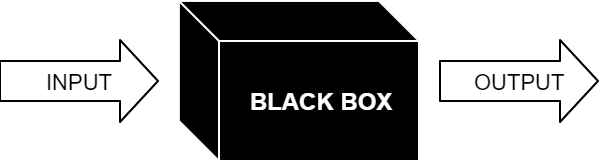
\includegraphics[width=80mm]{images/black-box.png}
		\caption{Phương pháp kiểm tra Black Box}
	\end{figure}
\end{center}
\par
Ứng dụng của chúng tôi sẽ áp dụng phương pháp kiểm tra này để đánh giá SEO cho website mà người dùng nhập vào. Cụ thể, ứng dụng sẽ tìm đến và tải về mã nguồn trang web, sau đó phân tích các thông tin nhận được, so sánh với các tiêu chí mà chúng tôi quy ước sẵn và trả về giao diện hiển thị kết quả cho người dùng.
\par
Với thiết kế này, người dùng sẽ không cần phải có kiến thức về lập trình. Ứng dụng của chúng tôi sẽ thay người dùng làm việc đó. Do đó mang lại trải nghiệm thuận tiện cho người dùng.
\par
Tuy nhiên, với giải pháp này, ứng dụng của chúng tôi sẽ xuất hiện vài khuyết điểm. Do không biết được mã nguồn chính xác của trang web, nên đôi khi trình phân tích mã nguồn của chúng tôi sẽ không ổn định, dẫn đến việc đánh giá sẽ không được chính xác hoàn toàn. Đối với các trang web được sinh ra bằng JavaScript, hiện tại thư viện phân tích mã nguồn của chúng tôi không thể tải về được cú pháp, do đó không thể kiểm tra được những trang web thuộc loại này.
\par
Nhìn chung, với việc áp dụng phương pháp kiểm tra trang web theo cơ chế black box sẽ mang đến trải nghiệm thuận tiện cho người dùng ứng dụng của chúng tôi.
\section{Kịch bản người dùng}
Chúng tôi xây dựng nên kịch bản của ứng dụng dành cho người dùng dựa trên mô hình MTV (Model - Template - View) của Django. Chúng tôi sử dụng sơ đồ bên dưới để trình bày về mô hình ứng dụng của chúng tôi.
\begin{center}
	\begin{figure}[!ht]
		\centering
		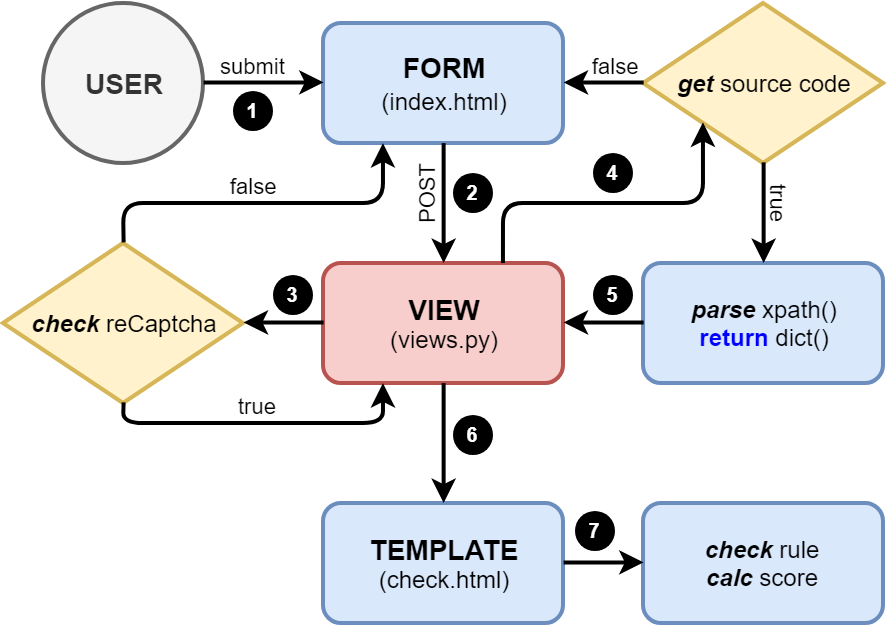
\includegraphics[width=120mm]{images/kich-ban-nguoi-dung.png}
		\caption{Kịch bản người dùng}
	\end{figure}
\end{center}
\begin{enumerate}
	\item Người dùng truy cập vào trang chủ của ứng dụng được lưu ở file \textbf{\texttt{index.html}}, tại đây hiển thị thẻ \textbf{\texttt{input}} để người dùng nhập url website cần kiểm tra.
	\item Khi người dùng bấm vào nút gửi, form sẽ gửi tín hiệu về \textbf{\texttt{VIEW}} với giao thức \textbf{\texttt{POST}}.
	\item Tại đây, chúng tôi có hàm để kiểm tra xem người dùng đã xác thực reCaptcha chưa. Nếu đúng, sẽ đi tiếp đến bước kế tiếp. Ngược lại, chúng tôi sẽ chuyển hướng người dùng về lại trang chủ và thông báo lỗi xác thực reCaptcha.
	\item Khi việc kiểm tra reCaptcha thành công, chúng tôi sẽ tiến hành truy vấn đến liên kết mà người dùng nhập vào, sau đó lấy nội dung source code bằng cách sữ dụng thư viện \textbf{\texttt{requests}}. Tuy nhiên, sẽ có trường hợp liên kết url của người dùng nhập vào bị sai, hoặc vì một lý do nào đó mà thư viện của chúng tôi không thể lấy source code được. Do đó, chúng tôi sử dụng cấu trúc \textbf{\texttt{try/except}} và trả về \textbf{\texttt{false}} nếu liên kết gặp lỗi.
	\item Tại đây, sau khi đã lấy được nội dung source code của trang web, chúng tôi cần định dạng lại bằng thư viện \textbf{\texttt{lxml}} để có thể thực hiện các toán tử \textbf{\texttt{xpath}} phân tích các thành phần trang web từ source code. Chúng tôi khai báo biến \textbf{\texttt{value}} với kiểu dữ liệu là \textbf{\texttt{dict()}} để lưu trữ kết quả sau khi phân tích, với mỗi tiêu chí đánh giá tương ứng với mỗi khóa riêng biệt trong biến \textbf{\texttt{value}}. Sau hàm xử lý này, biến \textbf{\texttt{value}} được trả về để tiếp tục quá trình triển khai trong ứng dụng.
	\item Sau khi nhận được dữ liệu về các yếu tố cần đánh giá, tiếp theo ứng dụng của chúng tôi sẽ truyền những giá trị này sang phía giao diện. Cụ thể, phần giao diện đảm nhiệm xử lý những dữ liệu này nằm ở file \textbf{\texttt{check.html}}.
	\item Với từng giá trị nhận được, chúng tôi sử dụng các thẻ hỗ trợ của Django để tiến hành so sánh với những tiêu chí về đánh giá web. Sau cùng, dựa trên những kết quả so sánh, chúng tôi sẽ sử dụng JavaScript để tính toán điểm số cho trang web dựa trên trọng số và hiển thị lên giao diện người dùng.
\end{enumerate}
\section{Giao diện người dùng}
Chúng tôi sử dụng tính kế thừa giao diện trong Django để thiết kế nên mô hình cho ứng dụng của mình. Ngoài ra, để tạo giao diện đa nền tảng, tối ưu với các thiết bị di động, chúng tôi sử dụng Bootstrap để quản lý tính responsive cho trang web. Bên cạnh đó, chúng tôi sử dụng Font Awesome để hiển thị icon trong trang web.
\par
Trong dụ án của chúng tôi, sẽ có hai phần ứng dụng con.
\begin{itemize}
	\item Checkweb: đây là ứng dụng trọng tâm cho dự án của chúng tôi, nơi chúng tôi xây dựng các hàm kiểm tra và đánh giá SEO cho trang web người dùng cần kiểm tra.
	\item Tips: sẽ là nơi chúng tôi đăng những bài viết về các tiêu chuẩn SEO, ứng dụng này chủ yếu là nhận truy vấn của người dùng và hiển thị giao diện web.
\end{itemize}
\subsubsection{base.html}
Đây là bộ khung cho ứng dụng, được chia thành ba khối cơ bản là \textbf{\texttt{title}} chứa tiêu đề, \textbf{\texttt{content}} chứa nội dung, \textbf{\texttt{script}} chứa các mã JavaScript.
\subsubsection{header.html, footer.html}
Hai file giao diện này có nội dung là hiển thị thanh menu ở đầu trang web và thông tin về dự án ở cuối trang. Thay vì được viết trực tiếp trong file \textbf{\texttt{base.html}}, chúng tôi chia nhỏ từng phần ra để code của chúng tôi được cấu trúc rõ ràng hơn. Sau cùng, chúng được \textbf{\texttt{include}} lại vào file \textbf{\texttt{base.html}} tại vị trí tương ứng cần hiển thị.
\subsubsection{index.html}
File này đóng vai trò là trang chủ trong ứng dụng. Chúng tôi hiển thị một form để người dùng nhập vào URL cần kiểm tra.
\par
Để bảo vệ website chúng tôi tránh liên tục spam truy vấn đến các trang web khác. Chúng tôi sử dụng phương thức POST cho form và sử dụng thêm reCAPTCHA nhằm xác thực người dùng.
\subsubsection{about.html, contact.html}
Hiển thị phần giới thiệu về ứng dụng của chúng tôi đến người dùng và thông tin liên hệ.
\subsubsection{check.html}
Trang này chúng tôi dùng để hiện thị thông tin được phân tích từ website của người dùng nhập vào. Kết quả sẽ được hiển thị bằng thẻ \textbf{\texttt{table}} gồm các cột:
\begin{itemize}
	\item Tiêu chí: Hiển thị các mục mà chúng tôi xem xét trang web người dùng, như là tiêu đề, mô tả và các thẻ khác.
	\item Kết quả: Sử dụng icon từ Font Awesome để cho người dùng biết tiêu chí đó có đạt yêu cầu hay không. Nếu đạt yêu cầu thì sẽ hiển thị icon có dấu tích xanh lá, ngược lại trang web hiển thị dấu x đỏ.
	\item Chi tiết: Mục này chúng tôi dùng để liệt kê ra nội dung được lấy từ trang web của người dùng, ví dụ như nội dung của thẻ tiêu đề, mô tả, hình ảnh\ldots
\end{itemize}
\par
Ngoài ra, chúng tôi sử dụng đoạn JavaScript để tính toán điểm cho website dựa trên kết quả kiểm tra, màu sắc sẽ thay đổi theo từng thang điểm:
\begin{itemize}
	\item $[80, 100]$: Màu xanh lá.
	\item $[50, 80)$: Màu vàng.
	\item $[0, 50)$: Màu đỏ.
\end{itemize}
\par
Nút Trở lại được đặt ở cuối bảng cho phép người dùng quay lại trang chủ để có thể kiểm tra trang web khác.
\section{Bảng đánh giá các tiêu chí SEO}
\begin{table}[!ht]
	\centering
	\begin{tabular}{|c|c|l|}
		\hline
		\textbf{Tiêu chí} & \textbf{Trọng số} & \textbf{Chi tiết}\\
		\hline
		Tiêu đề & 5 & Độ dài lớn hơn 0 và nhỏ hơn 65\\
		\hline
		Mô tả & 5 & Độ dài lớn hơn 0 và nhỏ hơn 160\\
		\hline
		Favicon & 5 & Có ảnh favicon trong trang web\\
		\hline
		Robots & 5 & Có thuộc tính robots trong trang web\\
		\hline
		Thẻ h1 & 5 & Có thẻ h1 trong trang web\\
		\hline
		Thẻ h2 & 4 & Có thẻ h2 trong trang web\\
		\hline
		Robots.txt & 5 & Có liên kết robots.txt trong trang web\\
		\hline
		Sitemap & 5 & Có liên kết sitemap trong trang web\\
		\hline
		Lỗi liên kết & 5* & Không có lỗi liên kết trong trang web\\
		\hline
		CSS nội tuyến & 3 & Không có thuộc tính CSS nội tuyến trong trang web\\
		\hline
		Thuộc tính alt & 5* & Có thuộc tính alt trong hình ảnh\\
		\hline
	\end{tabular}
	\caption{Bảng đánh giá các tiêu chí SEO}
\end{table}
\par
Trọng số có ký hiệu `*' sẽ có giá trị dựa theo tỉ lệ, giá trị càng lớn nếu vi phạm càng nhiều và được quy về mức trọng số là 5.
\par
Công thức tính điểm: $\displaystyle\frac{tongtrongso - trongsovipham}{tongtrongso}*100$
% Hiện thực
\chapter{Hiện thực}
% Kết luận đánh giá
\chapter{Kết luận đánh giá}
Trong giải pháp được nêu ở phần trước, chúng tôi chưa áp dụng lưu trữ vào cơ sở dữ liệu, tính năng này chúng tôi sẽ cập nhật vào các phiên bản tiếp theo. Ngoài ra, những phần kiến thức nền tảng chúng tôi sẽ sớm bổ sung thêm chi tiết đi kèm với nhiều ví dụ hơn.
\\\par
Hiện tại, ứng dụng của chúng tôi đã được triển khai với phiên bản thử nghiệm, người dùng có thể truy cập và thử dùng vài tính năng mà chúng tôi đã phát triển.
\\\par
Website: \url{https://checkseo.herokuapp.com}
\\\par
Chúng tôi nhận các ý kiến phản hồi đóng góp qua email: \href{mailto:npthinh1996@gmail.com}{npthinh1996@gmail.com}
% Tài liệu thao khảo
\bibliography{refer}
\bibliographystyle{unsrt}
\end{document}